\documentclass[
    twocolumn,
    fontsize = 10pt,
    parskip = half+,
    headings = small,
    headwidth = text,
    footwidth = text,
]{scrartcl}

\usepackage{pdflscape}
\usepackage{pgfgantt}
\usepackage{pdflscape}
\usetikzlibrary{shapes,backgrounds, arrows, positioning, trees, shadows}
\usepackage{pgf}
\usepackage{pgfplots}
\pgfplotsset{compat=1.18}
\selectcolormodel{rgb}

\KOMAoptions{
 paper = A4,
 pagesize,
 % headlines = 1.1,
 % headsepline,
 DIV = calc,
}
\typearea{11}

%\usepackage{fontspec}
%\setmainfont{Roboto Condensed}

\usepackage[
  todonotes={textsize=footnotesize},
  commandnameprefix=ifneeded,
  ulem={normalem,normalbf}
]{changes}
\definechangesauthor[name={Khalil Ben Larbi}, color=green]{kbl}

\usepackage{amsmath}

\usepackage[
  detect-all
]{siunitx}

\usepackage[
  style = ieee,
  backend = biber,
  hyperref = true,
  backref = true,
  seconds = true,
  date = iso,
]{biblatex}

\addbibresource{bib/bibliography.bib}

\usepackage{xurl}

\usepackage[acronyms=true]{glossaries}

\usepackage[
    colorlinks=true,
    allcolors=,
]{hyperref}

\usepackage[
    capitalize,
    nameinlink,
    noabbrev,
]{cleveref}

\newcommand{\rftvector}[1]{\underline{#1}}
\newcommand{\rftmatrix}[1]{\underline{\underline{#1}}}
\newcommand{\rftquaternion}[1]{\boldsymbol{#1}}

\newacronym{dfg}{DFG}{Deutsche Forschungsgemeinschaft}

\newacronym{rfi}{RFI}{Chair of Space Informatics and Satellite Systems}
\newacronym{rtg}{RTG}{radioisotope thermoelectric generator}

\newacronym{jmu}{JMU}{Julius-Maximilians-Universität Würzburg}

\newglossaryentry{cubesat}{
    name = CubeSat,
    description = {A small satellite following the form factor defined by the CubeSat Design Specification}
}

\makeglossaries

\title{Chair of Space Informatics and Satellite Systems Scientific Writing Guidelines}
\subtitle{Turning Humans into Space Scientists since 2003}
\author{
    \begin{minipage}[t]{.8\textwidth}
        \centering
         Mohamed Khalil Ben-Larbi, Markus Huwald
    \end{minipage}
}
\date{\today}

\begin{document}
\twocolumn[
\begin{@twocolumnfalse}

\maketitle

\begin{abstract}
Following the title, the abstract is the \textbf{second} most frequently read part of a scientific paper.
It informs about the general content and determines the paper's relevance for the reader.
It is good practice to write the abstract when writing the paper is \textbf{finished} in a way that it condenses and summarizes the content of the paper.
Only start writing the abstract when all required research and work has been finished.
Make the abstract one paragraph without reference and use about \numrange{200}{500} words.
Be sure to only draw conclusions and make only statements that are included in the paper.
Keep the text of the abstract in present tense.
A good approach to drafting an abstract is to start by summarizing  each section of the paper in \numrange{1}{2} sentences.
\end{abstract}
\end{@twocolumnfalse}
]
% Table of contents to be removed!
\tableofcontents
\newpage
%+++++++++++++++++++++++++++++++++++++++++++++++++++++++++++++++++++++++++++++++
%+++++++++++++++++++++++++++++++++++++++++++++++++++++++++++++++++++++++++++++++
\part{Preparing for Writing}
%+++++++++++++++++++++++++++++++++++++++++++++++++++++++++++++++++++++++++++++++
%+++++++++++++++++++++++++++++++++++++++++++++++++++++++++++++++++++++++++++++++
This part outlines the process involved in preparing to write a publication, including scientific reports, conference papers, or journal articles. 
It incudes all the preliminary steps you must go through \textbf{before} starting the actual writing of the paper.

%===============================================================================
\section{Publishing: The Questions of Why, What, and for Whom?}
%===============================================================================
The key considerations in the publishing process are: the rationale behind publishing (Why), the essence of what is to be published (What), and the identification of the target audience (for Whom). 

\textbf{Why} would we like to publish?
\begin{itemize}
    \item Disseminating research findings to the wider community?
    \item Soliciting feedback to refine and enhance the research?
    \item Clarifying and solidifying my research through peer scrutiny?
    \item Fulfilling academic requirements (e.g. my master thesis, my dissertation)?
    \item Achieving recognition and creating an impact in the scientific community?
    \item I want a "safe" paper and do not care about the impact? (Is this a good motivation?)
\end{itemize}

\textbf{What} would we like to publish?
\begin{itemize}
    \item Focus on addressing a research question rather than attempting to cover an entire project.
    \item Do I have a clear research gap?
    \item Novel and original?
    \item Internationally relevant? Beyond the specific context of my  study?
    \item Do I need permission? 
\end{itemize}

\textbf{Whom} would we like to address with our publication?
\begin{itemize}
    \item Communication needs an address. Knowing the audience simplifies both writing and publishing significantly!
    \item Who is interested in my topic?
    \item Who are the 10 people/departments I want to make sure they read my work?
\end{itemize}

%===============================================================================
\section{Define Authorship}
%===============================================================================
Criteria for authorship and acknowledgements according to \Gls{dfg} guidelines. 

%===============================================================================
\section{Set up a Paper Plan}
%===============================================================================
Create a detailed roadmap that includes the estimated time needed and the number of weeks required for each step below, taking into account the time available per week (add a 20\% buffer). 
As a rule of thumb,  a serious paper generally requires a minimum of four months. 
The project management appendix builds a solid basis for this task. 
\begin{enumerate}
    \item \textbf{Preparation}: define paper topic (includes drafting ideas and conducting thourough reserach) , target audience, paper type, journal, coauthors
    \item \textbf{Writing}: define objectives, structure and title. Write all paper sections including figs, tables and references. Collaborate with co-authors
    \item \textbf{Self-edit}: improve clarity, logic, style. Shorten paper. Special focus on Journal guidelines. 
    \item \textbf{Internal review}: ask colleagues to comment on your paper and implement changes. Perform language check. 
    \item \textbf{Submission}: final revision. prepare documents for submission
\end{enumerate}

Efficiency strategies such as keeping the paper concise, allocating more time per week, and delegating tasks to co-authors can help reduce the overall time. 

%+++++++++++++++++++++++++++++++++++++++++++++++++++++++++++++++++++++++++++++++
%+++++++++++++++++++++++++++++++++++++++++++++++++++++++++++++++++++++++++++++++
\part{Write the Paper}
%+++++++++++++++++++++++++++++++++++++++++++++++++++++++++++++++++++++++++++++++
%+++++++++++++++++++++++++++++++++++++++++++++++++++++++++++++++++++++++++++++++

This part outlines the writing process for a research paper. 
It offers overarching principles for scientific writing and provides detailed guidelines for the essential components of a research paper, including the title, abstract, core sections (Introduction, Methods, Results, Discussion), and supplementary elements (Appendices, References, etc.).

%===============================================================================
\section{Efficient Writing}
%===============================================================================
Start writing. Don't wait for the "right moment". 
It will never come! Writing brings clarity. 
Time and mood will follow. 
Cultivate the habit of writing regularly.
Short, frequent writing sessions of \numrange{30}{60} minutes daily are generally far more productive than attempting to compensate with single, longer session each week or month.

\begin{itemize}
    \item  \textbf{Small steps}: Break down large tasks into smaller, manageable ones. Create 30 min writing tasks.  Apply the Pareto principle: focus on the 20\% of tasks that will yield 80\% of results.
    \item \textbf{Prioritise}: Set aside dedicated time blocks in your calendar for writing. Minimize distractions by closing your door, and turning off emails and phone notifications.
    \item \textbf{Brevity}: Manage expectations and avoid the trap of perfectionism. Draft your thoughts briefly before fully articulating them. Keep it short!
    \item \textbf{Clarity}: Recognize that while a few readers might delve into the complexities and details, most seek a general understanding and will not invest excessive time in deciphering intricate details. To accommodate this, organize your paragraphs around central statements. Structure your paper in a way that allows for selective navigation, ensuring that the intellectual journey is clear and straightforward.  
\end{itemize}

%===============================================================================
\section{Define Objectives and Structure}
%===============================================================================
%------------------------------------------------------------------------------	
\subsection{Establishing a hypothesis}
%------------------------------------------------------------------------------	
Usually, a research hypothesis is driving your research. 
It is a precise, testable (or measurable) statement of the predicted outcome of the study. 
It further is a statement that introduces research goals and proposes an expected result. 
A hypothesis could be "rockets can be used to lift payloads into space". 
The research goals will follow subsequently: "definition of a correlation between rocket exhaust velocity and rocket acceleration" and "definition of a metric for calculation of payload masses that can be launched into orbit". 
Establishing such a hypothesis includes:
\begin{itemize}
    \item Stating the importance of the problem. Why does your research matter?
    \item Outlining the current situation regarding the problem by citing the literature. How did others evaluate the problem? 
    \item Evaluating the current situation (advantages/disadvantages). What approaches did other researchers already use? What results did they get?
    \item Identifying the gaps. Why isn't the work of other researchers sufficient for solving your problem? 
    \item Emphasizing the importance of the proposed research and how the gaps will be addressed. Why is "filling that gap" so important?
    \item Stating the research problem/questions.
    \item Stating the hypotheses briefly.
\end{itemize}

%------------------------------------------------------------------------------	
\subsection{Structuring the Paper}
%------------------------------------------------------------------------------	
When structuring a scientific paper, consider the following key sections: 
\begin{itemize}
    \item \textbf{Index}: this section is crucial for indexing the paper. It typically includes title, abstract, keywords, author
    \item \textbf{Main body}:  The structure of the main body may vary depending on the discipline and the type of paper. However, for research papers, the most common and recommended structure is the \textbf{IMRAD} format, which stands for Introduction, Methods, Results, and Discussion (plus Conclusion). This format provides a clear and logical flow of information.
    \item \textbf{References}:This section should include all the bibliographic references, acknowledgments, any appendices, and author biographies if required. It's essential for crediting sources and providing additional context or data.
\end{itemize} 

Define a clear and logical structure at the beginning of your writing process. Adhering closely to the IMRAD format is advisable for research papers.  Choose informative headings rather than creative ones. Well-crafted headings should be sufficient for a reader to understand the main points of the paper. Utilize subheadings, especially in the Methods, Results, and Discussion sections, to organize content and guide the reader through your paper.

%------------------------------------------------------------------------------	
\section{Title}
%------------------------------------------------------------------------------	
\begin{itemize}
    \item Most frequently read part of the paper
    \item most readers read only the title. The paper is only read if the titles captures the reader's interest
\end{itemize}
A title’s foremost purpose is to convey the content of the paper as accurately and concisely (with the fewest possible words) as possible.  
It serves not only as an elegant summary of the paper's subject but also plays a vital role in indexing and retrieval.
In essence, the title functions as the \textsl{business card} of the paper, providing a snapshot of the research within. 

\begin{itemize}
    \item include main keywords that reflect the content of the paper
    \item Title is a label, not necessarily a full grammatical sentence
    \item Understandable when read in isolation
    \item Short, informative, and includes subject of the study
    \item do not use fancy wordings or metaphors
    \item do not use too general titles (e.g. "spacecraft attitude control at TU Berlin")
    \item avoid too long and complicated titles
    \item avoid waste words (e.g. "a", "the", "study on", etc.) if possible
\end{itemize}

%------------------------------------------------------------------------------	
\section{Introduction}
%------------------------------------------------------------------------------	
The introduction informs the reader about the paper subject and context.
It helps understanding objectives and results. 
Note that if the problem is not well  understood, no one is interested in the solution. 
The introduction should include
\begin{itemize}
    \item Background: what is the overall problem?
    \item Motivation: why is it important?
    \item State-of-the-Art: what has been done before?
    \item Knowledge gaps: what is currently missing?
    The is the most important part of the introduction.
    \item Objectives: what is the paper doing?
    \item Definitions: what \textsl{unusual} terminology is the paper using?
\end{itemize}

\begin{figure}[h]
    \centering
    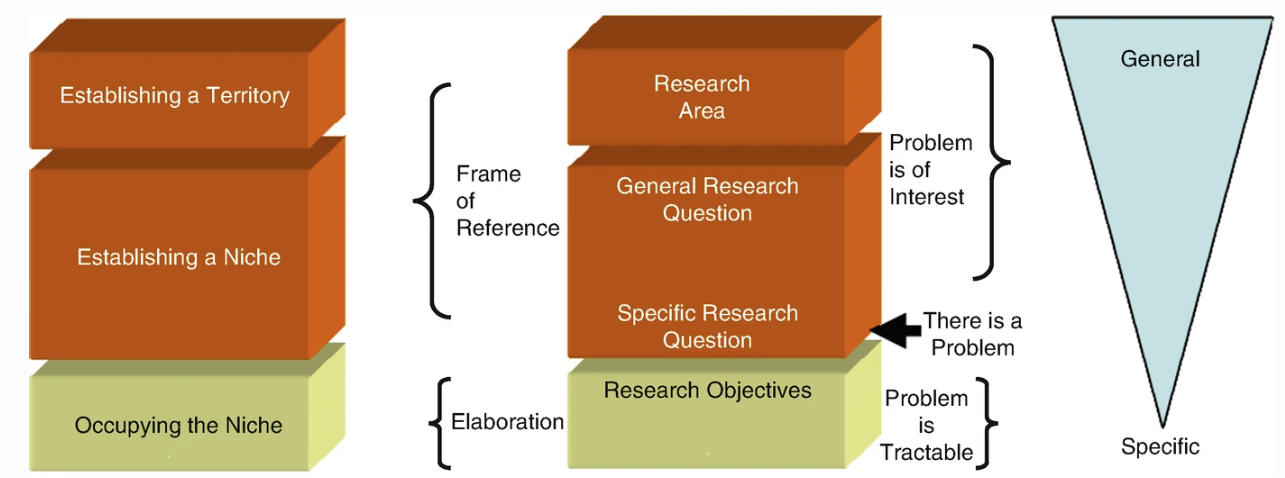
\includegraphics[width=1.0\linewidth]{pics/research_question.PNG}
    \caption{Flow of ideas from the general to the specific~\cite{Nundy.2022}}
    \label{fig: research question}
\end{figure}

%------------------------------------------------------------------------------	
\section{Methods}
%------------------------------------------------------------------------------	
This section elucidates the framework upon which the study is constructed, providing a comprehensive overview of the theoretical approach and experimental design.
Key objectives include:
\begin{itemize}
    \item Outlining the study's theoretical and experimental design to ensure the \textbf{replicability} of the research
    \item Ensuring the methods described are robust enough to guarantee the \textbf{validity} of the results
\end{itemize}

Reviewers examine the method section thoroughly.
A clear and reproducible methodology is a primary criterion for scientific rigor.
Ambiguity in this section can compromise the reliability of the results and often leads to the rejection of the paper.

Guidelines
\begin{itemize}
    \item Articulate the steps taken to achieve the objectives
    \item Include detailed description of models, tools, equipment, data collection
    \item Present the information in logical, chronological order facilitating easy follow-through (step by step)
    \item Be precise and concise.
    Strike a balance between referring relevant literature and explaining in detail
    \item Do not mix up methods and results
    \item Do not be vague.
    Provide exact numbers where possible
\end{itemize}

%------------------------------------------------------------------------------	
\section{Results}
%------------------------------------------------------------------------------	
The Results section is where you showcase your contribution of new knowledge to the scientific world.
While the Introduction and Methods sections explain why and how you arrived at these findings, the Results section presents them clearly.
It's distinct from the Discussion section, which interprets their meaning.
It's essential to distinguish between raw data – the factual information, figures from experiments and observations – and the results, which are statements based on this data that answer your research questions.
Key Points for the Results Section:

\begin{itemize}
    \item \textbf{Consistency and Relevance}: Ensure consistency throughout this section. Regularly revisit your objectives to ensure that you're fulfilling what was initially promised. The results presented should have a direct correlation with the objectives and research questions of your study. 
    \item \textbf{Data Presentation}: Present data that is representative, not repetitive. Opt for selected data that highlights your findings rather than including everything you gathered. 
    \item \textbf{Structured Approach}: Ideally, structure your results to follow your objectives step by step. Utilize headings and subheadings to guide the reader through your findings.
    \item \textbf{Clarity and Brevity}: Write in a sequential manner, being concise and precise. Avoid verbosity. The focus should be on clear communication of your findings. 
    \item \textbf{Use of Visuals}: Leverage figures and tables to present your data. Determine which data can be effectively displayed in figures and tables for a clearer understanding. Highlight the main message of each visual element without repeating the information verbatim. 
    \item Do not introduce new methods in the Results section. 
    \item Avoid discussing or interpreting the results; this is reserved for the Discussion section. 
    \item Do not present results that do not align with your objectives.
\end{itemize}

%------------------------------------------------------------------------------	
\section{Discussion}
%------------------------------------------------------------------------------	
In a research paper, data provides the raw information, and results offer specific facts in response to research questions. The Discussion section takes these elements further by delving into their interpretation. It connects your findings to the existing state of the art, which you initially introduced in the Introduction. This section is pivotal as it extends beyond presenting mere data or results; it contextualizes your findings within the broader spectrum of current knowledge. Here, you have the opportunity to underscore the wider significance of your work, offering insights that contribute to a larger conversation in your field. Writing the Discussion section demands a comprehensive understanding of existing literature and a nuanced interpretation of your results, making it both critical and challenging.

Key Elements of the Discussion Section are:
\begin{itemize}
    \item  \textbf{Principles and Generalizations}: Discuss the principles, relationships, and generalizations that emerge from your results. Focus on meaningful patterns or trends identified. 
    \item  \textbf{Unexpected Results}: Address any surprising findings, extreme observations, or lacking correlations. Explore potential reasons for these anomalies.  
    \item  \textbf{Critical Assessment}: Evaluate your methods and acknowledge any limitations that might affect the validity of your analysis. Discuss potential limitations transparently. 
   \item  \textbf{ Comparative Analysis}: Reflect on how your findings relate to previous studies in the field. Discuss reasons why your results might differ from past research. 
    \item  \textbf{Implications}: Consider the theoretical implications of your results and their practical applications. Suggest practical steps or applications based on your findings. 
\end{itemize}

%------------------------------------------------------------------------------	
\section{Conclusion}
%------------------------------------------------------------------------------	
In engineering and some other disciplines, the Conclusion is often integrated with the Discussion section.
Crafting the Conclusion:
\begin{itemize}
    \item Summarize Key Findings: Concisely restate the main findings of your research. 
    \item Take-Home Message: Clearly articulate the core message or insight that you want readers to take away from your study. This should be a distillation of your research's most significant insights or contributions.
    \item Future Directions (Optional): If appropriate, suggest areas for future research or potential developments that may stem from your work.
\end{itemize}

\printbibliography

\printglossaries
% Appendix
\appendix
\pagenumbering{roman}
% Manage your appendix
% use \input{appendix/tex_file_name} to add to the appendix

% Project management
\pagebreak
\onecolumn
\begin{landscape}
\section{Project Management}
%______________________________________________________________
% Work Breakdown Structure
% Breakdown of the tasks in individual work packages.
% Up to two levels of workpackages
%______________________________________________________________

\subsection{Work Breakdown Structure}

    \small
    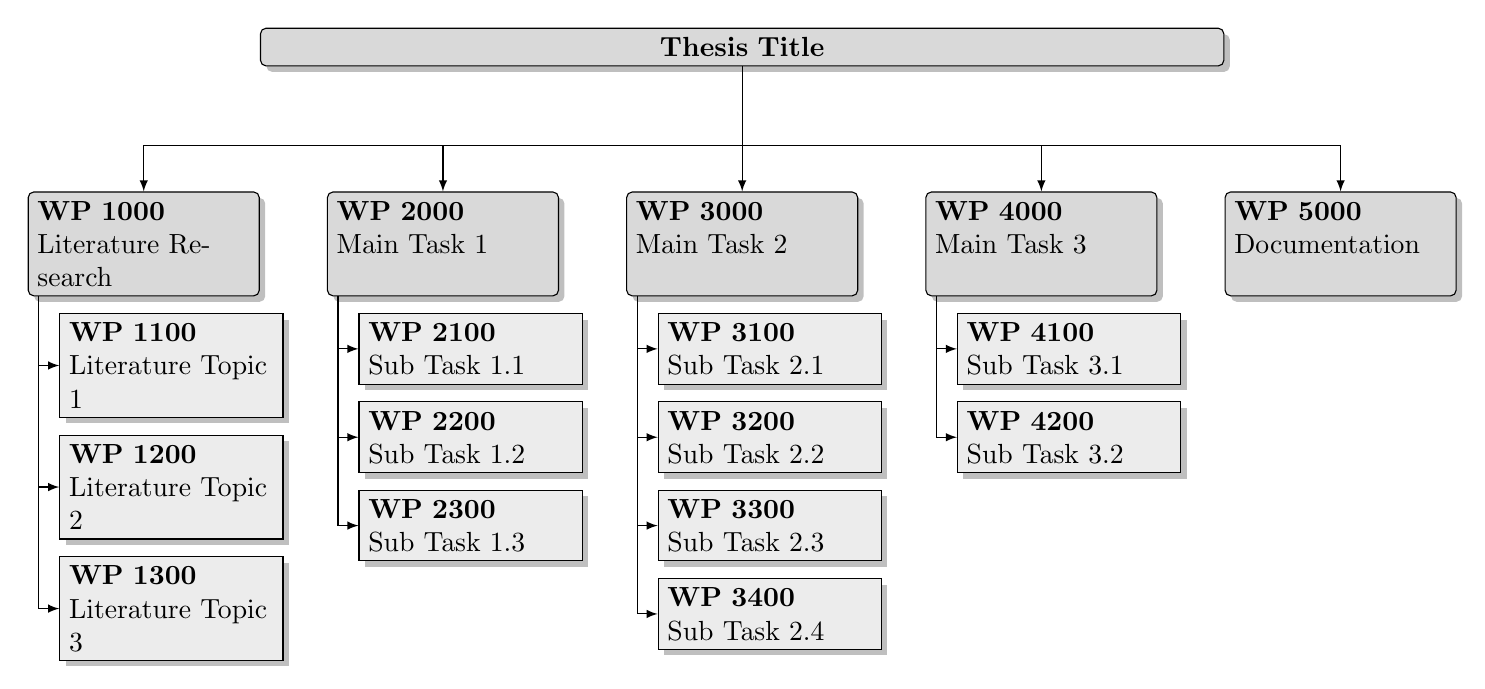
\begin{tikzpicture}[
        basic/.style   = {draw, text width=2.7cm, align=left, drop shadow, rectangle},
        root/.style    = {basic, text width=12cm, rounded corners=2pt, thin, align=center, fill=gray!30},
        level 2/.style = {basic, rounded corners=2pt, thin, fill=gray!30},
        level 3/.style = {basic, thin, fill=gray!15, text width=2.6cm},
        level 1/.style={sibling distance=38mm}, edge from parent fork down,
        edge from parent/.style={->,draw}, level distance=2.5cm,  >=latex]

    % root of the the initial tree, level 1
    \node[root] {\textbf{Thesis Title}}
    % The first level, as children of the initial tree
        child {node[level 2] (c1) {\textbf{WP~1000} \\ Literature Research}}
        child {node[level 2] (c2) {\textbf{WP~2000} \\ Main Task 1 \\ $~~$}}
        child {node[level 2] (c3) {\textbf{WP~3000} \\ Main Task 2 \\ $~~$}}
        child {node[level 2] (c4) {\textbf{WP~4000} \\ Main Task 3 \\ $~~$}}
        child {node[level 2] (c5) {\textbf{WP~5000} \\ Documentation \\ $~~$}};

    % The second level, relatively positioned nodes
    \begin{scope}[every node/.style={level 3}, node distance=6pt]
    \node [below=of c1, xshift=10pt] (c11) {\textbf{WP~1100} \\ Literature Topic 1};
    \node [below=of c11] (c12) {\textbf{WP~1200} \\ Literature Topic 2};
    \node [below=of c12] (c13) {\textbf{WP~1300} \\ Literature Topic 3};

    \node [below=of c2, xshift=10pt] (c21) {\textbf{WP~2100} \\ Sub Task 1.1};
    \node [below=of c21] (c22) {\textbf{WP~2200} \\ Sub Task 1.2};
    \node [below=of c22] (c23) {\textbf{WP~2300} \\ Sub Task 1.3};

    \node [below=of c3, xshift=10pt] (c31) {\textbf{WP~3100} \\ Sub Task 2.1};
    \node [below=of c31] (c32) {\textbf{WP~3200} \\ Sub Task 2.2};
    \node [below=of c32] (c33) {\textbf{WP~3300} \\ Sub Task 2.3};
    \node [below=of c33] (c34) {\textbf{WP~3400} \\ Sub Task 2.4};

    \node [below=of c4, xshift=10pt] (c41) {\textbf{WP~4100} \\ Sub Task 3.1};
    \node [below=of c41] (c42) {\textbf{WP~4200} \\ Sub Task 3.2};

    \end{scope}

    % lines from each level 1 node to every one of its "children"
    \foreach \value in {1,2,3}
        \draw[->] ([xshift=4pt]c1.south west) |- (c1\value.west);

    \foreach \value in {1,2,3}
        \draw[->] ([xshift=4pt]c2.south west) |- (c2\value.west);

    \foreach \value in {1,2,3,4}
        \draw[->] ([xshift=4pt]c3.south west) |- (c3\value.west);

    \foreach \value in {1,2}
        \draw[->] ([xshift=4pt]c4.south west) |- (c4\value.west);

    \end{tikzpicture}
    \normalsize

\end{landscape}

\begin{landscape}

%______________________________________________________________
% Gantt Chart
% Time line of the project
% Shows duration and chronological structure for each 
%  workpackage and project milestones
%______________________________________________________________
\subsection{Gantt Chart}
\definecolor{color_bar}{RGB}{0, 63, 137}
\definecolor{color_group}{RGB}{0, 37, 82}
\begin{center}
    \begin{ganttchart}[
        expand chart=.95\linewidth,
        vgrid,
        bar/.append style={fill=color_bar, draw=none},
        group/.append style={fill=color_group},
        group left shift=0,
        group right shift=0,
        group peaks tip position=0,
        group peaks height=.25,
        y unit chart = 0.445cm,
        group top shift=0.25,
        bar top shift=-0.1,
        bar height=0.6,
        milestone top shift=-0.1,
        milestone/.append style={xscale=0.5}]{1}{16}
        \gantttitle{Weeks}{16} \\
        \gantttitlelist{1,...,16}{1} \\

        \ganttgroup{WP 1000: Literature Research}{1}{5} \\
        \ganttbar{WP 1100: Literature Topic 1}{1}{3} \\
        \ganttbar{WP 1200: Literature Topic 2}{2}{4} \\
        \ganttbar{WP 1300: Literature Topic 3}{2}{5} \\
        \\
        \ganttgroup{WP 2000: Main Task 1}{4}{8} \\
        \ganttbar{WP 2100: Sub Task 1.1}{4}{6} \\
        \ganttbar{WP 2200: Sub Task 1.2}{6}{7} \\
        \ganttbar{WP 2300: Sub Task 1.3}{7}{8} \\
        \ganttmilestone{Milestone 1}{8} \\
        \\
        \ganttgroup{WP 3000: Main Task 2}{4}{11} \\
        \ganttbar{WP 3100: Sub Task 2.1}{4}{5} \\
        \ganttbar{WP 3200: Sub Task 2.2}{5}{6} \\
        \ganttbar{WP 3300: Sub Task 2.3}{6}{8} \\
        \ganttbar{WP 3400: Sub Task 2.4}{7}{11} \\
        \ganttmilestone{Milestone 2}{11} \\
        \\
        \ganttgroup{WP 4000: Main Task 3}{8}{12} \\
        \ganttbar{WP 4100: Sub Task 3.1}{8}{12} \\
        \ganttbar{WP 4200: Sub Task 3.2}{8}{12} \\
        \ganttmilestone{Milestone 3}{12} \\
        \\
        \ganttgroup{WP 5000: Documentation}{1}{16} \\
        \ganttmilestone{Draft}{12} \\
        \ganttmilestone{Submission}{16}
    \end{ganttchart}
\end{center}
\end{landscape}

%______________________________________________________________
% Work Package Description
% Detailed description of each workpackage
%______________________________________________________________

\subsection{Work Package Description}

\newcommand{\wpddate}{27.09.2021}
%%%%
% WP1000 - Literature Research
%%%%

\begin{table}[!h]
    \begin{center}
        \begin{tabular}{|p{.2\columnwidth}||p{.3\columnwidth}|p{.27\columnwidth}||p{.23\columnwidth}|}
            \hline
            \multicolumn{3}{|l||}{\textbf{}} & \multicolumn{1}{c|}{}\\
            \multicolumn{3}{|l||}{\textbf{}} & \multicolumn{1}{c|}{\textbf{WP 1100}}\\
            \multicolumn{3}{|l||}{\textbf{}} & \multicolumn{1}{c|}{}\\
            \hline\hline
            \textbf{Title} & \multicolumn{2}{p{.40\columnwidth}||}{\textbf{Literature Topic 1}}
            & \textbf{Page:} 1 of 1\\
            \hline
            \textbf{Responsible} & \multicolumn{2}{l||}{Ame Watson} & \textbf{Version:} 1.0\\
            \hline
            \multicolumn{3}{|l||}{} & \textbf{Date:} \wpddate\\
            \hline\hline
            \textbf{Start} & \multicolumn{2}{l||}{Week 1} & \\
            \hline
            \textbf{End} & \multicolumn{2}{l||}{Week 3} & \textbf{Duration}: 3 Weeks\\
            \hline\hline
            \textbf{Processed by} & \multicolumn{3}{l|}{Ame Watson}\\
            \hline\hline
            \multicolumn{4}{|p{.95\columnwidth}|}{\textbf{Goals:}}\\
            \multicolumn{4}{|p{.95\columnwidth}|}{$\bullet$ Gain knowledge about the literature research topic 1}\\
            \multicolumn{4}{|p{.95\columnwidth}|}{$\bullet$ Gain a deep understanding of the current state of the art on research topic 1}\\
            \multicolumn{4}{|p{.95\columnwidth}|}{}\\
            \multicolumn{4}{|p{.95\columnwidth}|}{\textbf{Input:}}\\
            \multicolumn{4}{|p{.95\columnwidth}|}{$\bullet$ Journal papers on literature topic 1}\\
            \multicolumn{4}{|p{.95\columnwidth}|}{$\bullet$ Conference papers on literature topic 1}\\
            \multicolumn{4}{|p{.95\columnwidth}|}{}\\
            \multicolumn{4}{|p{.95\columnwidth}|}{\textbf{Connections to other WPs:}}\\
            \multicolumn{4}{|p{.95\columnwidth}|}{}\\
            \multicolumn{4}{|p{.95\columnwidth}|}{\textbf{Tasks:}}\\
            \multicolumn{4}{|p{.95\columnwidth}|}{$\bullet$ Literature research literature topic 1}\\
            \multicolumn{4}{|p{.95\columnwidth}|}{}\\
            \multicolumn{4}{|p{.95\columnwidth}|}{\textbf{Results:}}\\
            \multicolumn{4}{|p{.95\columnwidth}|}{$\bullet$ Basic knowledge about literature topic 1}\\
            \multicolumn{4}{|p{.95\columnwidth}|}{$\bullet$ Deeper knowledge about literature topic 1}\\
            \hline
        \end{tabular}
    \end{center}
\end{table}

\clearpage

\begin{table}[!h]
    \begin{center}
        \begin{tabular}{|p{.2\columnwidth}||p{.3\columnwidth}|p{.27\columnwidth}||p{.23\columnwidth}|}
            \hline
            \multicolumn{3}{|l||}{\textbf{}} & \multicolumn{1}{c|}{}\\
            \multicolumn{3}{|l||}{\textbf{}} & \multicolumn{1}{c|}{\textbf{WP 1200}}\\
            \multicolumn{3}{|l||}{\textbf{}} & \multicolumn{1}{c|}{}\\
            \hline\hline
            \textbf{Title} & \multicolumn{2}{p{.40\columnwidth}||}{\textbf{Literature Topic 2}}
            & \textbf{Page:} 1 of 1\\
            \hline
            \textbf{Responsible} & \multicolumn{2}{l||}{Ame Watson} & \textbf{Version:} 1.0\\
            \hline
            \multicolumn{3}{|l||}{} & \textbf{Date:} \wpddate\\
            \hline\hline
            \textbf{Start} & \multicolumn{2}{l||}{Week 2} & \\
            \hline
            \textbf{End} & \multicolumn{2}{l||}{Week 4} & \textbf{Duration}: 3 Weeks\\
            \hline\hline
            \textbf{Processed by} & \multicolumn{3}{l|}{Ame Watson}\\
            \hline\hline
            \multicolumn{4}{|p{.95\columnwidth}|}{\textbf{Goals:}}\\
            \multicolumn{4}{|p{.95\columnwidth}|}{$\bullet$ Get insight into literature topic 2}\\
            \multicolumn{4}{|p{.95\columnwidth}|}{$\bullet$ Gather state-of-the-art information on literature topic 2}\\
            \multicolumn{4}{|p{.95\columnwidth}|}{}\\
            \multicolumn{4}{|p{.95\columnwidth}|}{\textbf{Input:}}\\
            \multicolumn{4}{|p{.95\columnwidth}|}{$\bullet$ Literature on literature topic 2}\\
            \multicolumn{4}{|p{.95\columnwidth}|}{$\bullet$ Literature on literature topic 2}\\
            \multicolumn{4}{|p{.95\columnwidth}|}{}\\
            \multicolumn{4}{|p{.95\columnwidth}|}{\textbf{Connections to other WPs:}}\\
            \multicolumn{4}{|p{.95\columnwidth}|}{}\\
            \multicolumn{4}{|p{.95\columnwidth}|}{\textbf{Tasks:}}\\
            \multicolumn{4}{|p{.95\columnwidth}|}{$\bullet$ Literature research on literature topic 2}\\
            \multicolumn{4}{|p{.95\columnwidth}|}{$\bullet$ Literature research on literature topic 2}\\
            \multicolumn{4}{|p{.95\columnwidth}|}{}\\
            \multicolumn{4}{|p{.95\columnwidth}|}{\textbf{Results:}}\\
            \multicolumn{4}{|p{.95\columnwidth}|}{$\bullet$ Basic knowledge on literature topic 2}\\
            \multicolumn{4}{|p{.95\columnwidth}|}{$\bullet$ Basic knowledge on literature topic 2 in general}\\
            \hline
        \end{tabular}
    \end{center}
\end{table}

\clearpage

\begin{table}[!h]
    \begin{center}
        \begin{tabular}{|p{.2\columnwidth}||p{.3\columnwidth}|p{.27\columnwidth}||p{.23\columnwidth}|}
            \hline
            \multicolumn{3}{|l||}{\textbf{}} & \multicolumn{1}{c|}{}\\
            \multicolumn{3}{|l||}{\textbf{}} & \multicolumn{1}{c|}{\textbf{WP 1300}}\\
            \multicolumn{3}{|l||}{\textbf{}} & \multicolumn{1}{c|}{}\\
            \hline\hline
            \textbf{Title} & \multicolumn{2}{p{.40\columnwidth}||}{\textbf{Literature Topic 3}}
            & \textbf{Page:} 1 of 1\\
            \hline
            \textbf{Responsible} & \multicolumn{2}{l||}{Ame Watson} & \textbf{Version:} 1.0\\
            \hline
            \multicolumn{3}{|l||}{} & \textbf{Date:} \wpddate\\
            \hline\hline
            \textbf{Start} & \multicolumn{2}{l||}{Week 2} & \\
            \hline
            \textbf{End} & \multicolumn{2}{l||}{Week 5} & \textbf{Duration}: 4 Weeks\\
            \hline\hline
            \textbf{Processed by} & \multicolumn{3}{l|}{Ame Watson}\\
            \hline\hline
            \multicolumn{4}{|p{.95\columnwidth}|}{\textbf{Goals:}}\\
            \multicolumn{4}{|p{.95\columnwidth}|}{$\bullet$ Get insight into literature topic 3, to be able to derive decisions and requirements about stuff}\\
            \multicolumn{4}{|p{.95\columnwidth}|}{}\\
            \multicolumn{4}{|p{.95\columnwidth}|}{\textbf{Input:}}\\
            \multicolumn{4}{|p{.95\columnwidth}|}{$\bullet$ Documentation of literature topic 3}\\
            \multicolumn{4}{|p{.95\columnwidth}|}{}\\
            \multicolumn{4}{|p{.95\columnwidth}|}{\textbf{Connections to other WPs:}}\\
            \multicolumn{4}{|p{.95\columnwidth}|}{$\bullet$ \textbf{WP 3200} Research for subsystems/units/parts/components}\\
            \multicolumn{4}{|p{.95\columnwidth}|}{$\bullet$ \textbf{WP 3200} Gather technical solutions for novel design}\\
            \multicolumn{4}{|p{.95\columnwidth}|}{}\\
            \multicolumn{4}{|p{.95\columnwidth}|}{\textbf{Tasks:}}\\
            \multicolumn{4}{|p{.95\columnwidth}|}{$\bullet$ Literature research on literature topic 3}\\            \multicolumn{4}{|p{.95\columnwidth}|}{}\\
            \multicolumn{4}{|p{.95\columnwidth}|}{\textbf{Results:}}\\
            \multicolumn{4}{|p{.95\columnwidth}|}{$\bullet$ Select technical solutions of literature topic 3 as proposal for thingy to be developed}\\
            \hline
        \end{tabular}
    \end{center}
\end{table}

\clearpage

%%%%
% WP2000 - Main Task 1
%%%%

\begin{table}[!h]
    \begin{center}
        \begin{tabular}{|p{.2\columnwidth}||p{.3\columnwidth}|p{.27\columnwidth}||p{.23\columnwidth}|}
            \hline
            \multicolumn{3}{|l||}{\textbf{}} & \multicolumn{1}{c|}{}\\
            \multicolumn{3}{|l||}{\textbf{}} & \multicolumn{1}{c|}{\textbf{WP 2100}}\\
            \multicolumn{3}{|l||}{\textbf{}} & \multicolumn{1}{c|}{}\\
            \hline\hline
            \textbf{Title} & \multicolumn{2}{p{.40\columnwidth}||}{\textbf{Sub Task 1.1}}
            & \textbf{Page:} 1 of 1\\
            \hline
            \textbf{Responsible} & \multicolumn{2}{l||}{Ame Watson} & \textbf{Version:} 1.0\\
            \hline
            \multicolumn{3}{|l||}{} & \textbf{Date:} \wpddate\\
            \hline\hline
            \textbf{Start} & \multicolumn{2}{l||}{Week 4} & \\
            \hline
            \textbf{End} & \multicolumn{2}{l||}{Week 6} & \textbf{Duration}: 3 Weeks\\
            \hline\hline
            \textbf{Processed by} & \multicolumn{3}{l|}{Ame Watson}\\
            \hline\hline
            \multicolumn{4}{|p{.95\columnwidth}|}{\textbf{Goals:}}\\
            \multicolumn{4}{|p{.95\columnwidth}|}{$\bullet$ Identify needs and characteristics for sub task 2.1}\\
            \multicolumn{4}{|p{.95\columnwidth}|}{$\bullet$ Identify requirements and expected performance}\\
            \multicolumn{4}{|p{.95\columnwidth}|}{$\bullet$ Identify constraints}\\
            \multicolumn{4}{|p{.95\columnwidth}|}{}\\
            \multicolumn{4}{|p{.95\columnwidth}|}{\textbf{Input:}}\\
            \multicolumn{4}{|p{.95\columnwidth}|}{$\bullet$ Documentation, haha }\\
            \multicolumn{4}{|p{.95\columnwidth}|}{$\bullet$ Documentation of other stuff xD}\\
            \multicolumn{4}{|p{.95\columnwidth}|}{}\\
            \multicolumn{4}{|p{.95\columnwidth}|}{\textbf{Connections to other WPs:}}\\
            \multicolumn{4}{|p{.95\columnwidth}|}{$\bullet$ \textbf{WP 1100} Input from the literature research}\\
            \multicolumn{4}{|p{.95\columnwidth}|}{}\\
            \multicolumn{4}{|p{.95\columnwidth}|}{\textbf{Tasks:}}\\
            \multicolumn{4}{|p{.95\columnwidth}|}{$\bullet$ Precisely define the thingy to be defined in sub task 2.1}\\
            \multicolumn{4}{|p{.95\columnwidth}|}{}\\
            \multicolumn{4}{|p{.95\columnwidth}|}{\textbf{Results:}}\\
            \multicolumn{4}{|p{.95\columnwidth}|}{$\bullet$ Requirements for development thingy}\\
            \multicolumn{4}{|p{.95\columnwidth}|}{$\bullet$ Furhter results}\\
            \hline
        \end{tabular}
    \end{center}
\end{table}

\clearpage

\begin{table}[!h]
    \begin{center}
        \begin{tabular}{|p{.2\columnwidth}||p{.3\columnwidth}|p{.27\columnwidth}||p{.23\columnwidth}|}
            \hline
            \multicolumn{3}{|l||}{\textbf{}} & \multicolumn{1}{c|}{}\\
            \multicolumn{3}{|l||}{\textbf{}} & \multicolumn{1}{c|}{\textbf{WP 2200}}\\
            \multicolumn{3}{|l||}{\textbf{}} & \multicolumn{1}{c|}{}\\
            \hline\hline
            \textbf{Title} & \multicolumn{2}{p{.40\columnwidth}||}{\textbf{Sub Task 1.2}}
            & \textbf{Page:} 1 of 1\\
            \hline
            \textbf{Responsible} & \multicolumn{2}{l||}{Ame Watson} & \textbf{Version:} 1.0\\
            \hline
            \multicolumn{3}{|l||}{} & \textbf{Date:} \wpddate\\
            \hline\hline
            \textbf{Start} & \multicolumn{2}{l||}{Week 6} & \\
            \hline
            \textbf{End} & \multicolumn{2}{l||}{Week 7} & \textbf{Duration}: 2 Weeks\\
            \hline\hline
            \textbf{Processed by} & \multicolumn{3}{l|}{Ame Watson}\\
            \hline\hline
            \multicolumn{4}{|p{.95\columnwidth}|}{\textbf{Goals:}}\\
            \multicolumn{4}{|p{.95\columnwidth}|}{$\bullet$ Compare the current state of the stuff to the previous defined requirements}\\
            \multicolumn{4}{|p{.95\columnwidth}|}{$\bullet$ Additional Goal}\\
            \multicolumn{4}{|p{.95\columnwidth}|}{}\\
            \multicolumn{4}{|p{.95\columnwidth}|}{\textbf{Input:}}\\
            \multicolumn{4}{|p{.95\columnwidth}|}{$\bullet$ Results from WPXXXX}\\
            \multicolumn{4}{|p{.95\columnwidth}|}{$\bullet$ Input from WPXXXX}\\
            \multicolumn{4}{|p{.95\columnwidth}|}{}\\
            \multicolumn{4}{|p{.95\columnwidth}|}{\textbf{Connections to other WPs:}}\\
            \multicolumn{4}{|p{.95\columnwidth}|}{$\bullet$ \textbf{WP XXXX} Connection to this workpkg}\\
            \multicolumn{4}{|p{.95\columnwidth}|}{$\bullet$ \textbf{WP XXXX} Connection to this workpkg}\\
            \multicolumn{4}{|p{.95\columnwidth}|}{}\\
            \multicolumn{4}{|p{.95\columnwidth}|}{\textbf{Tasks:}}\\
            \multicolumn{4}{|p{.95\columnwidth}|}{$\bullet$ Task-A of Sub Task 1.2}\\
            \multicolumn{4}{|p{.95\columnwidth}|}{$\bullet$ Task-B of Sub Task 1.2}\\
            \multicolumn{4}{|p{.95\columnwidth}|}{}\\
            \multicolumn{4}{|p{.95\columnwidth}|}{\textbf{Results:}}\\
            \multicolumn{4}{|p{.95\columnwidth}|}{$\bullet$ Result of Sub Task 1.2}\\
            \hline
        \end{tabular}
    \end{center}
\end{table}

\clearpage

\begin{table}[!h]
    \begin{center}
        \begin{tabular}{|p{.2\columnwidth}||p{.3\columnwidth}|p{.27\columnwidth}||p{.23\columnwidth}|}
            \hline
            \multicolumn{3}{|l||}{\textbf{}} & \multicolumn{1}{c|}{}\\
            \multicolumn{3}{|l||}{\textbf{}} & \multicolumn{1}{c|}{\textbf{WP 2300}}\\
            \multicolumn{3}{|l||}{\textbf{}} & \multicolumn{1}{c|}{}\\
            \hline\hline
            \textbf{Title} & \multicolumn{2}{p{.40\columnwidth}||}{\textbf{Sub Task 1.3}}
            & \textbf{Page:} 1 of 1\\
            \hline
            \textbf{Responsible} & \multicolumn{2}{l||}{Ame Watson} & \textbf{Version:} 1.0\\
            \hline
            \multicolumn{3}{|l||}{} & \textbf{Date:} \wpddate\\
            \hline\hline
            \textbf{Start} & \multicolumn{2}{l||}{Week 6} & \\
            \hline
            \textbf{End} & \multicolumn{2}{l||}{Week 8} & \textbf{Duration}: 2 Weeks\\
            \hline\hline
            \textbf{Processed by} & \multicolumn{3}{l|}{Ame Watson}\\
            \hline\hline
            \multicolumn{4}{|p{.95\columnwidth}|}{\textbf{Goals:}}\\
            \multicolumn{4}{|p{.95\columnwidth}|}{$\bullet$ Goal-A of Sub Task 1.3}\\
            \multicolumn{4}{|p{.95\columnwidth}|}{$\bullet$ Goal-B of Sub Task 1.3}\\
            \multicolumn{4}{|p{.95\columnwidth}|}{}\\
            \multicolumn{4}{|p{.95\columnwidth}|}{\textbf{Input:}}\\
            \multicolumn{4}{|p{.95\columnwidth}|}{$\bullet$ Results from WPXXXX}\\
            \multicolumn{4}{|p{.95\columnwidth}|}{$\bullet$ Input from WPXXXX}\\
            \multicolumn{4}{|p{.95\columnwidth}|}{}\\
            \multicolumn{4}{|p{.95\columnwidth}|}{\textbf{Connections to other WPs:}}\\
            \multicolumn{4}{|p{.95\columnwidth}|}{$\bullet$ \textbf{WP XXXX} connection to this workpg}\\
            \multicolumn{4}{|p{.95\columnwidth}|}{$\bullet$ \textbf{WP XXXX} connection to this workpg}\\
            \multicolumn{4}{|p{.95\columnwidth}|}{}\\
            \multicolumn{4}{|p{.95\columnwidth}|}{\textbf{Tasks:}}\\
            \multicolumn{4}{|p{.95\columnwidth}|}{$\bullet$ Task-A of Sub Task 1.3}\\
            \multicolumn{4}{|p{.95\columnwidth}|}{$\bullet$ Task-B of Sub Task 1.3}\\
            \multicolumn{4}{|p{.95\columnwidth}|}{}\\
            \multicolumn{4}{|p{.95\columnwidth}|}{\textbf{Results:}}\\
            \multicolumn{4}{|p{.95\columnwidth}|}{$\bullet$ Result of Sub Task 1.3}\\
            \hline
        \end{tabular}
    \end{center}
\end{table}

\clearpage

%%%%
% WP3000 - Main Task 2
%%%%

\begin{table}[!h]
    \begin{center}
        \begin{tabular}{|p{.2\columnwidth}||p{.3\columnwidth}|p{.27\columnwidth}||p{.23\columnwidth}|}
            \hline
            \multicolumn{3}{|l||}{\textbf{}} & \multicolumn{1}{c|}{}\\
            \multicolumn{3}{|l||}{\textbf{}} & \multicolumn{1}{c|}{\textbf{WP 3100}}\\
            \multicolumn{3}{|l||}{\textbf{}} & \multicolumn{1}{c|}{}\\
            \hline\hline
            \textbf{Title} & \multicolumn{2}{p{.40\columnwidth}||}{\textbf{Sub Task 2.1}}
            & \textbf{Page:} 1 of 1\\
            \hline
            \textbf{Responsible} & \multicolumn{2}{l||}{Ame Watson} & \textbf{Version:} 1.0\\
            \hline
            \multicolumn{3}{|l||}{} & \textbf{Date:} \wpddate\\
            \hline\hline
            \textbf{Start} & \multicolumn{2}{l||}{Week 4} & \\
            \hline
            \textbf{End} & \multicolumn{2}{l||}{Week 5} & \textbf{Duration}: 2 Weeks\\
            \hline\hline
            \textbf{Processed by} & \multicolumn{3}{l|}{Ame Watson}\\
            \hline\hline
            \multicolumn{4}{|p{.95\columnwidth}|}{\textbf{Goals:}}\\
            \multicolumn{4}{|p{.95\columnwidth}|}{$\bullet$ Goal of Sub Task 2.1}\\
            \multicolumn{4}{|p{.95\columnwidth}|}{}\\
            \multicolumn{4}{|p{.95\columnwidth}|}{\textbf{Input:}}\\
            \multicolumn{4}{|p{.95\columnwidth}|}{$\bullet$ Input-A for Sub Task 2.1}\\
            \multicolumn{4}{|p{.95\columnwidth}|}{$\bullet$ Input-B for Sub Task 2.1}\\
            \multicolumn{4}{|p{.95\columnwidth}|}{$\bullet$ Input-C for Sub Task 2.1}\\
            \multicolumn{4}{|p{.95\columnwidth}|}{}\\
            \multicolumn{4}{|p{.95\columnwidth}|}{\textbf{Connections to other WPs:}}\\
            \multicolumn{4}{|p{.95\columnwidth}|}{$\bullet$ \textbf{WP XXXX} connection to this workpkg}\\
            \multicolumn{4}{|p{.95\columnwidth}|}{$\bullet$ \textbf{WP XXXX} connection to this workpkg}\\
            \multicolumn{4}{|p{.95\columnwidth}|}{$\bullet$ \textbf{WP XXXX} connection to this workpkg}\\
            \multicolumn{4}{|p{.95\columnwidth}|}{}\\
            \multicolumn{4}{|p{.95\columnwidth}|}{\textbf{Tasks:}}\\
            \multicolumn{4}{|p{.95\columnwidth}|}{$\bullet$ Task of Sub Task 2.1}\\
            \multicolumn{4}{|p{.95\columnwidth}|}{}\\
            \multicolumn{4}{|p{.95\columnwidth}|}{\textbf{Results:}}\\
            \multicolumn{4}{|p{.95\columnwidth}|}{$\bullet$ Result-A of Sub Task 2.1}\\
            \multicolumn{4}{|p{.95\columnwidth}|}{$\bullet$ Result-B of Sub Task 2.1}\\
            \hline
        \end{tabular}
    \end{center}
\end{table}

\clearpage

\begin{table}[!h]
    \begin{center}
        \begin{tabular}{|p{.2\columnwidth}||p{.3\columnwidth}|p{.27\columnwidth}||p{.23\columnwidth}|}
            \hline
            \multicolumn{3}{|l||}{\textbf{}} & \multicolumn{1}{c|}{}\\
            \multicolumn{3}{|l||}{\textbf{}} & \multicolumn{1}{c|}{\textbf{WP 3200}}\\
            \multicolumn{3}{|l||}{\textbf{}} & \multicolumn{1}{c|}{}\\
            \hline\hline
            \textbf{Title} & \multicolumn{2}{p{.40\columnwidth}||}{\textbf{Sub Task 2.2}}
            & \textbf{Page:} 1 of 1\\
            \hline
            \textbf{Responsible} & \multicolumn{2}{l||}{Ame Watson} & \textbf{Version:} 1.0\\
            \hline
            \multicolumn{3}{|l||}{} & \textbf{Date:} \wpddate\\
            \hline\hline
            \textbf{Start} & \multicolumn{2}{l||}{Week 5} & \\
            \hline
            \textbf{End} & \multicolumn{2}{l||}{Week 6} & \textbf{Duration}: 2 Weeks\\
            \hline\hline
            \textbf{Processed by} & \multicolumn{3}{l|}{Ame Watson}\\
            \hline\hline
            \multicolumn{4}{|p{.95\columnwidth}|}{\textbf{Goals:}}\\
            \multicolumn{4}{|p{.95\columnwidth}|}{$\bullet$ Goal-A of Sub Task 2.2}\\
            \multicolumn{4}{|p{.95\columnwidth}|}{$\bullet$ Goal-B of Sub Task 2.2}\\
            \multicolumn{4}{|p{.95\columnwidth}|}{}\\
            \multicolumn{4}{|p{.95\columnwidth}|}{\textbf{Input:}}\\
            \multicolumn{4}{|p{.95\columnwidth}|}{$\bullet$ Input-A for Sub Task 2.2}\\
            \multicolumn{4}{|p{.95\columnwidth}|}{$\bullet$ Input-B for Sub Task 2.2}\\
            \multicolumn{4}{|p{.95\columnwidth}|}{}\\
            \multicolumn{4}{|p{.95\columnwidth}|}{\textbf{Connections to other WPs:}}\\
            \multicolumn{4}{|p{.95\columnwidth}|}{$\bullet$ \textbf{WP XXXX/XXXX} connection to these workpkgs}\\
            \multicolumn{4}{|p{.95\columnwidth}|}{$\bullet$ \textbf{WP XXXX/XXXX} connection to these workpkgs}\\
            \multicolumn{4}{|p{.95\columnwidth}|}{}\\
            \multicolumn{4}{|p{.95\columnwidth}|}{\textbf{Tasks:}}\\
            \multicolumn{4}{|p{.95\columnwidth}|}{$\bullet$ Task-A of Sub Task 2.2}\\
            \multicolumn{4}{|p{.95\columnwidth}|}{$\bullet$ Task-B of Sub Task 2.2}\\
            \multicolumn{4}{|p{.95\columnwidth}|}{}\\
            \multicolumn{4}{|p{.95\columnwidth}|}{\textbf{Results:}}\\
            \multicolumn{4}{|p{.95\columnwidth}|}{$\bullet$ Result-A of Sub Task 2.2}\\
            \multicolumn{4}{|p{.95\columnwidth}|}{$\bullet$ Result-B of Sub Task 2.2}\\
            \hline
        \end{tabular}
    \end{center}
\end{table}

\clearpage

\begin{table}[!h]
    \begin{center}
        \begin{tabular}{|p{.2\columnwidth}||p{.3\columnwidth}|p{.27\columnwidth}||p{.23\columnwidth}|}
            \hline
            \multicolumn{3}{|l||}{\textbf{}} & \multicolumn{1}{c|}{}\\
            \multicolumn{3}{|l||}{\textbf{}} & \multicolumn{1}{c|}{\textbf{WP 3300}}\\
            \multicolumn{3}{|l||}{\textbf{}} & \multicolumn{1}{c|}{}\\
            \hline\hline
            \textbf{Title} & \multicolumn{2}{p{.40\columnwidth}||}{\textbf{Sub Task 2.3}}
            & \textbf{Page:} 1 of 1\\
            \hline
            \textbf{Responsible} & \multicolumn{2}{l||}{Ame Watson} & \textbf{Version:} 1.0\\
            \hline
            \multicolumn{3}{|l||}{} & \textbf{Date:} \wpddate\\
            \hline\hline
            \textbf{Start} & \multicolumn{2}{l||}{Week 6} & \\
            \hline
            \textbf{End} & \multicolumn{2}{l||}{Week 8} & \textbf{Duration}: 3 Weeks\\
            \hline\hline
            \textbf{Processed by} & \multicolumn{3}{l|}{Ame Watson}\\
            \hline\hline
            \multicolumn{4}{|p{.95\columnwidth}|}{\textbf{Goals:}}\\
            \multicolumn{4}{|p{.95\columnwidth}|}{$\bullet$ Goal of Sub Task 2.3}\\
            \multicolumn{4}{|p{.95\columnwidth}|}{}\\
            \multicolumn{4}{|p{.95\columnwidth}|}{\textbf{Input:}}\\
            \multicolumn{4}{|p{.95\columnwidth}|}{$\bullet$ Input for Sub Task 2.1}\\
            \multicolumn{4}{|p{.95\columnwidth}|}{}\\
            \multicolumn{4}{|p{.95\columnwidth}|}{\textbf{Connections to other WPs:}}\\
            \multicolumn{4}{|p{.95\columnwidth}|}{}\\
            \multicolumn{4}{|p{.95\columnwidth}|}{\textbf{Tasks:}}\\
            \multicolumn{4}{|p{.95\columnwidth}|}{$\bullet$ Task of Sub Task 2.3}\\
            \multicolumn{4}{|p{.95\columnwidth}|}{}\\
            \multicolumn{4}{|p{.95\columnwidth}|}{\textbf{Results:}}\\
            \multicolumn{4}{|p{.95\columnwidth}|}{$\bullet$ Result of Sub Task 2.3}\\
            \hline
        \end{tabular}
    \end{center}
\end{table}

\clearpage

\begin{table}[!h]
    \begin{center}
        \begin{tabular}{|p{.2\columnwidth}||p{.3\columnwidth}|p{.27\columnwidth}||p{.23\columnwidth}|}
            \hline
            \multicolumn{3}{|l||}{\textbf{}} & \multicolumn{1}{c|}{}\\
            \multicolumn{3}{|l||}{\textbf{}} & \multicolumn{1}{c|}{\textbf{WP 3400}}\\
            \multicolumn{3}{|l||}{\textbf{}} & \multicolumn{1}{c|}{}\\
            \hline\hline
            \textbf{Title} & \multicolumn{2}{p{.40\columnwidth}||}{\textbf{Sub Task 2.4}}
            & \textbf{Page:} 1 of 1\\
            \hline
            \textbf{Responsible} & \multicolumn{2}{l||}{Ame Watson} & \textbf{Version:} 1.0\\
            \hline
            \multicolumn{3}{|l||}{} & \textbf{Date:} \wpddate\\
            \hline\hline
            \textbf{Start} & \multicolumn{2}{l||}{Week 7} & \\
            \hline
            \textbf{End} & \multicolumn{2}{l||}{Week 11} & \textbf{Duration}: 5 Weeks\\
            \hline\hline
            \textbf{Processed by} & \multicolumn{3}{l|}{Ame Watson}\\
            \hline\hline
            \multicolumn{4}{|p{.95\columnwidth}|}{\textbf{Goals:}}\\
            \multicolumn{4}{|p{.95\columnwidth}|}{$\bullet$ Goal of Sub Task 2.4}\\
            \multicolumn{4}{|p{.95\columnwidth}|}{}\\
            \multicolumn{4}{|p{.95\columnwidth}|}{\textbf{Input:}}\\
            \multicolumn{4}{|p{.95\columnwidth}|}{$\bullet$ Input-A for Sub Task 2.4}\\
            \multicolumn{4}{|p{.95\columnwidth}|}{$\bullet$ Input-B for Sub Task 2.4}\\
            \multicolumn{4}{|p{.95\columnwidth}|}{}\\
            \multicolumn{4}{|p{.95\columnwidth}|}{\textbf{Connections to other WPs:}}\\
            \multicolumn{4}{|p{.95\columnwidth}|}{}\\
            \multicolumn{4}{|p{.95\columnwidth}|}{\textbf{Tasks:}}\\
            \multicolumn{4}{|p{.95\columnwidth}|}{$\bullet$ Task of Sub Task 2.4}\\
            \multicolumn{4}{|p{.95\columnwidth}|}{}\\
            \multicolumn{4}{|p{.95\columnwidth}|}{\textbf{Results:}}\\
            \multicolumn{4}{|p{.95\columnwidth}|}{$\bullet$ Result of Sub Task 3.4}\\
            \hline
        \end{tabular}
    \end{center}
\end{table}

\clearpage

%%%%
% WP4000 - Main Task 3
%%%%

\begin{table}[!h]
    \begin{center}
        \begin{tabular}{|p{.2\columnwidth}||p{.3\columnwidth}|p{.27\columnwidth}||p{.23\columnwidth}|}
            \hline
            \multicolumn{3}{|l||}{\textbf{}} & \multicolumn{1}{c|}{}\\
            \multicolumn{3}{|l||}{\textbf{}} & \multicolumn{1}{c|}{\textbf{WP 4100}}\\
            \multicolumn{3}{|l||}{\textbf{}} & \multicolumn{1}{c|}{}\\
            \hline\hline
            \textbf{Title} & \multicolumn{2}{p{.40\columnwidth}||}{\textbf{Sub Task 3.1}}
            & \textbf{Page:} 1 of 1\\
            \hline
            \textbf{Responsible} & \multicolumn{2}{l||}{Ame Watson} & \textbf{Version:} 1.0\\
            \hline
            \multicolumn{3}{|l||}{} & \textbf{Date:} \wpddate\\
            \hline\hline
            \textbf{Start} & \multicolumn{2}{l||}{Week 8} & \\
            \hline
            \textbf{End} & \multicolumn{2}{l||}{Week 12} & \textbf{Duration}: 5 Weeks\\
            \hline\hline
            \textbf{Processed by} & \multicolumn{3}{l|}{Ame Watson}\\
            \hline\hline
            \multicolumn{4}{|p{.95\columnwidth}|}{\textbf{Goals:}}\\
            \multicolumn{4}{|p{.95\columnwidth}|}{$\bullet$ Goal of Sub Task 3.1}\\
            \multicolumn{4}{|p{.95\columnwidth}|}{}\\
            \multicolumn{4}{|p{.95\columnwidth}|}{\textbf{Input:}}\\
            \multicolumn{4}{|p{.95\columnwidth}|}{$\bullet$ Input for Sub Task 3.1}\\
            \multicolumn{4}{|p{.95\columnwidth}|}{}\\
            \multicolumn{4}{|p{.95\columnwidth}|}{\textbf{Connections to other WPs:}}\\
            \multicolumn{4}{|p{.95\columnwidth}|}{}\\
            \multicolumn{4}{|p{.95\columnwidth}|}{\textbf{Tasks:}}\\
            \multicolumn{4}{|p{.95\columnwidth}|}{$\bullet$ Task of Sub Task 3.1}\\
            \multicolumn{4}{|p{.95\columnwidth}|}{}\\
            \multicolumn{4}{|p{.95\columnwidth}|}{\textbf{Results:}}\\
            \multicolumn{4}{|p{.95\columnwidth}|}{$\bullet$ Result of Sub Task 3.1}\\
            \hline
        \end{tabular}
    \end{center}
\end{table}

\clearpage

\begin{table}[!h]
    \begin{center}
        \begin{tabular}{|p{.2\columnwidth}||p{.3\columnwidth}|p{.27\columnwidth}||p{.23\columnwidth}|}
            \hline
            \multicolumn{3}{|l||}{\textbf{}} & \multicolumn{1}{c|}{}\\
            \multicolumn{3}{|l||}{\textbf{}} & \multicolumn{1}{c|}{\textbf{WP 4200}}\\
            \multicolumn{3}{|l||}{\textbf{}} & \multicolumn{1}{c|}{}\\
            \hline\hline
            \textbf{Title} & \multicolumn{2}{p{.40\columnwidth}||}{\textbf{Sub Task 3.2}}
            & \textbf{Page:} 1 of 1\\
            \hline
            \textbf{Responsible} & \multicolumn{2}{l||}{Ame Watson} & \textbf{Version:} 1.0\\
            \hline
            \multicolumn{3}{|l||}{} & \textbf{Date:} \wpddate\\
            \hline\hline
            \textbf{Start} & \multicolumn{2}{l||}{Week 8} & \\
            \hline
            \textbf{End} & \multicolumn{2}{l||}{Week 12} & \textbf{Duration}: 5 Weeks\\
            \hline\hline
            \textbf{Processed by} & \multicolumn{3}{l|}{Ame Watson}\\
            \hline\hline
            \multicolumn{4}{|p{.95\columnwidth}|}{\textbf{Goals:}}\\
            \multicolumn{4}{|p{.95\columnwidth}|}{$\bullet$ Goal-A of Sub Task 3.2}\\
            \multicolumn{4}{|p{.95\columnwidth}|}{$\bullet$ Goal-B of Sub Task 3.2}\\
            \multicolumn{4}{|p{.95\columnwidth}|}{}\\
            \multicolumn{4}{|p{.95\columnwidth}|}{\textbf{Input:}}\\
            \multicolumn{4}{|p{.95\columnwidth}|}{$\bullet$ Input for Sub Task 3.2}\\
            \multicolumn{4}{|p{.95\columnwidth}|}{}\\
            \multicolumn{4}{|p{.95\columnwidth}|}{\textbf{Connections to other WPs:}}\\
            \multicolumn{4}{|p{.95\columnwidth}|}{}\\
            \multicolumn{4}{|p{.95\columnwidth}|}{\textbf{Tasks:}}\\
            \multicolumn{4}{|p{.95\columnwidth}|}{$\bullet$ Task-A of Sub Task 3.2}\\
            \multicolumn{4}{|p{.95\columnwidth}|}{$\bullet$ Task-B of Sub Task 3.2}\\
            \multicolumn{4}{|p{.95\columnwidth}|}{}\\
            \multicolumn{4}{|p{.95\columnwidth}|}{\textbf{Results:}}\\
            \multicolumn{4}{|p{.95\columnwidth}|}{$\bullet$ Results of Sub Task 3.2}\\
            \hline
        \end{tabular}
    \end{center}
\end{table}

\clearpage

%%%%
% WP5000 - Documentation
%%%%

\begin{table}[!h]
    \begin{center}
        \begin{tabular}{|p{.2\columnwidth}||p{.3\columnwidth}|p{.27\columnwidth}||p{.23\columnwidth}|}
            \hline
            \multicolumn{3}{|l||}{\textbf{}} & \multicolumn{1}{c|}{}\\
            \multicolumn{3}{|l||}{\textbf{}} & \multicolumn{1}{c|}{\textbf{WP 5000}}\\
            \multicolumn{3}{|l||}{\textbf{}} & \multicolumn{1}{c|}{}\\
            \hline\hline
            \textbf{Title} & \multicolumn{2}{p{.40\columnwidth}||}{\textbf{Documentation}}
            & \textbf{Page:} 1 of 1\\
            \hline
            \textbf{Responsible} & \multicolumn{2}{l||}{Ame Watson} & \textbf{Version:} 1.0\\
            \hline
            \multicolumn{3}{|l||}{} & \textbf{Date:} \wpddate\\
            \hline\hline
            \textbf{Start} & \multicolumn{2}{l||}{Week 1} & \\
            \hline
            \textbf{End} & \multicolumn{2}{l||}{Week 16} & \textbf{Duration}: 16 Weeks\\
            \hline\hline
            \textbf{Processed by} & \multicolumn{3}{l|}{Ame Watson}\\
            \hline\hline
            \multicolumn{4}{|p{.95\columnwidth}|}{\textbf{Goals:}}\\
            \multicolumn{4}{|p{.95\columnwidth}|}{$\bullet$ Documentation of work on all WPs}\\
            \multicolumn{4}{|p{.95\columnwidth}|}{}\\
            \multicolumn{4}{|p{.95\columnwidth}|}{\textbf{Input:}}\\
            \multicolumn{4}{|p{.95\columnwidth}|}{$\bullet$ WPs 1000-4000}\\
            \multicolumn{4}{|p{.95\columnwidth}|}{}\\
            \multicolumn{4}{|p{.95\columnwidth}|}{\textbf{Connections to other WPs:}}\\
            \multicolumn{4}{|p{.95\columnwidth}|}{}\\
            \multicolumn{4}{|p{.95\columnwidth}|}{\textbf{Tasks:}}\\
            \multicolumn{4}{|p{.95\columnwidth}|}{$\bullet$ Produce draft}\\
            \multicolumn{4}{|p{.95\columnwidth}|}{$\bullet$ Revise draft}\\
            \multicolumn{4}{|p{.95\columnwidth}|}{}\\
            \multicolumn{4}{|p{.95\columnwidth}|}{\textbf{Results:}}\\
            \multicolumn{4}{|p{.95\columnwidth}|}{$\bullet$ Final documentation}\\
            \hline
        \end{tabular}
    \end{center}
\end{table}

\clearpage


\end{document}

